\section{Results}
\label{sec:results}

The expected signal significance for s$\lq$, d$\lq$ and non-res production, and their combination, is presented in Fig.~\ref{fig:heatmapssignificance}. Here, the significance is shown as a heat map in a two dimensional plane of $g_U$ versus $M_U$, considering exclusive couplings to left-handed currents, \textit{i.e.} ${\rm BR}(\lq \to \bq\,\tau)=\tfrac12$. The dashed lines show the contours of constant signal significance. The $1.69 \sigma$ contour represents exclusion at 95\% confidence level, and the 3-5$\sigma$ contours represent potential discovery. The grey band defines the set of $\set{M_{U},g_{U}}$ values that can explain the $\Bm$-meson anomalies, $C_U\sim 0.01$ for this scenario. The estimates are performed under the conditions for the second run, RUN-II, of the LHC ($\sqrt{s} = 13 \tev$ and $L = 137 \fb^{-1}$). We find that the d$\lq$ interpretation plot (Figure ~\ref{fig:heatmapssignificance} second from the top) does not depend on $g_{U}$, which is expected due to d$\lq$ production arising exclusively from interactions with gluons. For this reason, the d$\lq$ production process provides the best mode for discovery when $g_{U}$ is small. On the other hand, the non-res channel is more sensitive to changes in the coupling parameter $g_U$, as its production cross-section depends on $g_{U}^{4}$. Therefore, the non-res production process provides the best mode for discovery when $g_{U}$ is large. These results confirm the expectations from previous analyses (see for instance~\cite{Schmaltz:2018nls}), in the sense that the d$\lq$ and non-res processes complement each other nicely at low and high $g_{U}$ scenarios. The s$\lq$ channel combines features from both the d$\lq$ and non-res channels, in principle making it an interesting option to explore different scenarios and gain a better understanding of $\lq$ properties, but the evolution of the signal significance in the full phase space is more complicated as it involves resonant $\lq$ production with a cross-section that depends non-trivially on $M_{U}$, $g_{U}$, and the $\lq$ coupling to gluons. However, Fig.~\ref{fig:heatmapssignificance} shows that the s$\lq$ production process can provide complementary and competitive sensitivity to the non-res and d$\lq$ processes, in certain parts of the phase space.

\begin{figure}[t]
    \centering
       \begin{subfigure}[b]{.48\linewidth}
            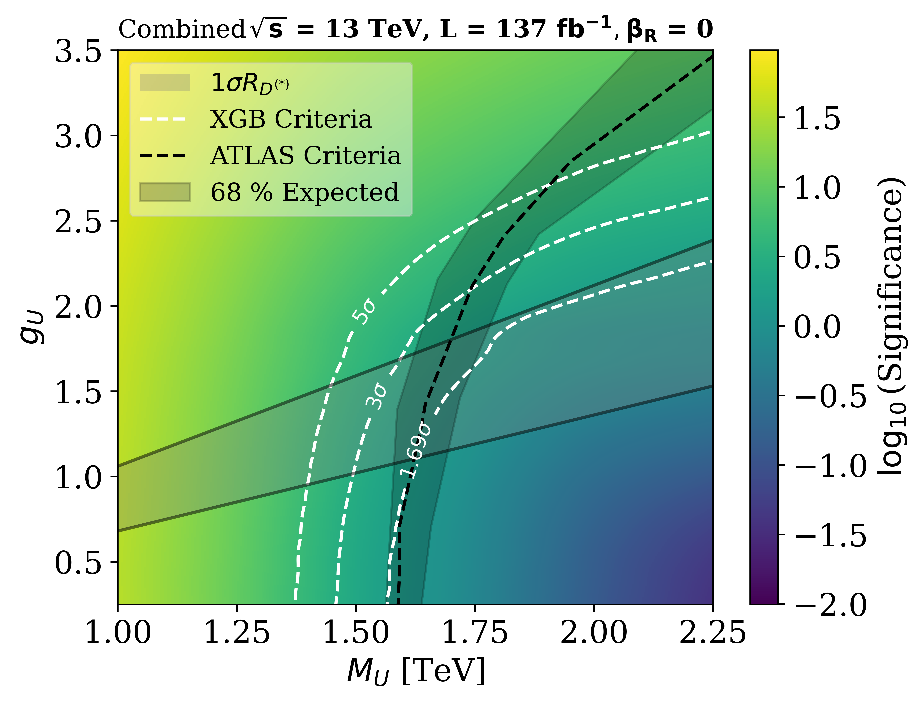
\includegraphics[height=5.8cm]{Images/Significance/Significance_Heatmap_13TeV_L137_all_combined_woRHC.pdf}
        \end{subfigure}    
       \begin{subfigure}[b]{.48\linewidth}
            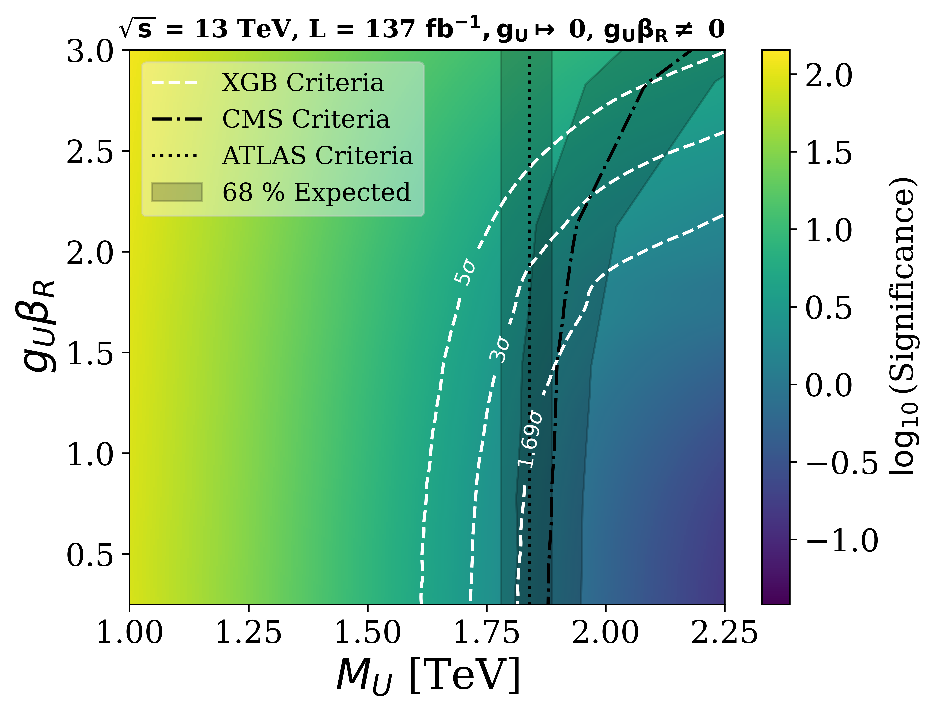
\includegraphics[height=5.8cm]{Images/Significance/Significance_CMS_Comparison_13TeV_L137_all_combined_woRHC.pdf}
        \end{subfigure}    
    \caption{The top (bottom) panel shows signal significance comparison with ATLAS~\cite{ATLAS_7A} (CMS and ATLAS~\cite{ LQS_CMS_2022_results_comparison, ATLAS_Vertical_Line}) background only hypothesis, for the combination of all channels, with uniquely coupling to left-handed (right-handed) currents. The estimates are performed at $\sqrt{s} = 13 \tev$ and $137 \fb^{-1}$.}
    \label{fig:heatmapscomparingcms}
    %It also includes a comparison with CMS results (report CMS-PAS-EXO-19-016)
\end{figure}

The top panel of Fig.~\ref{fig:heatmapscomparingcms} presents the sensitivity of all signal production processes combined, and compares our expected exclusion region with the latest one from the ATLAS Collaboration~\cite{ATLAS_7A}. The comparison suggests that our proposed analysis strategy provides better sensitivity than current methods being carried out at ATLAS, especially at large values of $g_U$. In particular, we find that with the $\textrm{pp}$ data already available from RUN-II, our expected exclusion curves begin to probe solutions to the B-anomalies for $\lq$ masses up to $2.25\tev$.


Fig.~\ref{fig:heatmapscomparingcms} shows the expected signal significance considering ${\rm BR}(\lq \to \bq\,\tau) = 1$, in order to compare our analysis with the corresponding results from the CMS~\cite{LQS_CMS_2022_results_comparison} and ATLAS~\cite{ATLAS_Vertical_Line} Collaborations. Let us emphasize again that ${\rm BR}(\lq \to \bq\,\tau)$ depends on $\beta_R$, as illustrated on the top panel of Fig.~\ref{fig:branching_ratios}. Thus, although the ${\rm BR}(\lq \to \bq\,\tau) = 1$ scenario is a possible physical case, it does not solve the observed anomalies in the $R_{D^{(*)}}$ ratios, as it corresponds to the case where LQs couple exclusively to right-handed currents.

With this in mind, the scenario studied by CMS in~\cite{LQS_CMS_2022_results_comparison} considers couplings only to left-handed currents, setting artificially the condition ${\rm BR}(\lq \to \bq\,\tau) = 1$. In order to compare, we scale the efficiency$\times$acceptance of our selection criteria for $\beta_R=0$, by a factor of 2.0 for s$\lq$ and 4.0 for d$\lq$. According to Fig.~\ref{fig:heatmapscomparingcms}, the ML approach that we have followed again suggests an optimisation of the signal and background separation, having the potential of improving the regions of exclusion (1.69 $\sigma$) with respect to that of CMS. In the bottom panel of the Figure we have also included a similar exclusion by ATLAS~\cite{ATLAS_Vertical_Line}. However, since ATLAS only considers d$\lq$ production in the analysis, the results are not entirely comparable, so are included only as a reference. 

\begin{figure}[t]
    \centering
    \begin{subfigure}[b]{0.495\textwidth}
            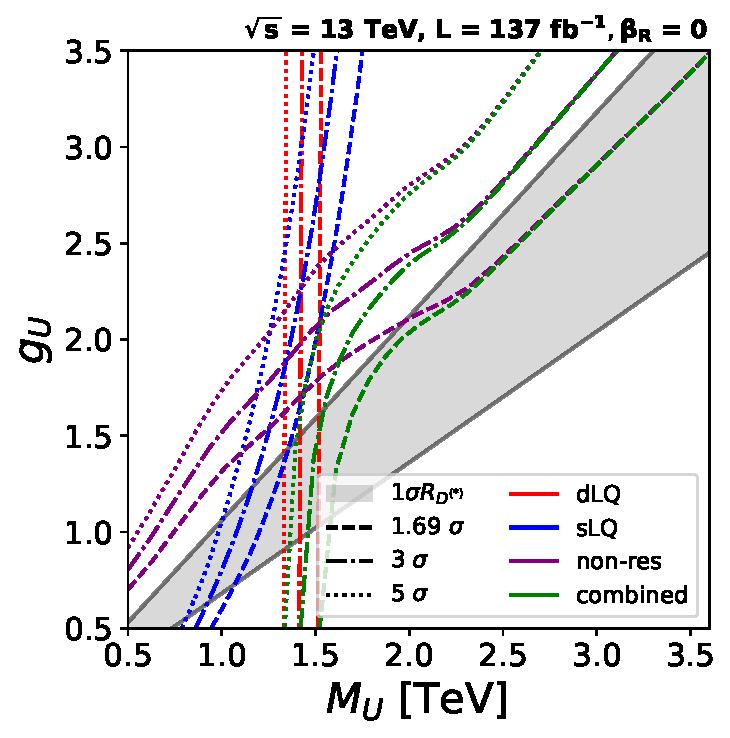
\includegraphics[height=6.3cm]{Images/Significance/Significance_Curves_13TeV_L137_summary_all_sigmas_woRHC.pdf}
    \end{subfigure}
    \begin{subfigure}[b]{0.495\textwidth}
            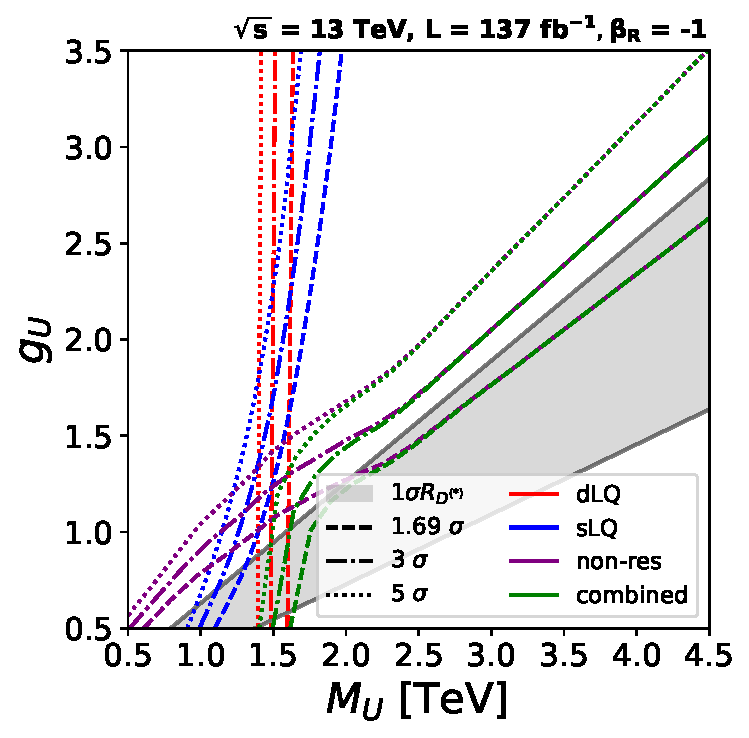
\includegraphics[height=6.3cm]{Images/Significance/Significance_Curves_13TeV_L137_summary_all_sigmas_wRHC.pdf}
    \end{subfigure}
    \caption{Signal significance for different coupling scenarios and $\lq$ masses for all channels. This plot summarizes our results with $\beta_{R} = 0$ (without right-handed currents) and $\beta_{R} = -1$ (maximally coupled to right-handed currents). The estimates are performed at $\sqrt{s} = 13 \tev$ and $137 \fb^{-1}$.}
    \label{fig:significance137ifb}
\end{figure}
We now turn to the role of $\beta_R$, and our capacity of probing the regions solving the B-meson anomalies. Fig.~\ref{fig:significance137ifb} shows the maximum significant contours, under LHC RUN-II conditions, for the different $\lq$ production mechanisms and their combination, considering scenarios with only left-handed currents ($\beta_R=0$, top) and with maximal right-handed currents ($\beta_R=-1$, bottom). We find a noticeable improvement in signal significance in all channels when taking $\beta_R=-1$, as is expected from the increase in ${\rm BR}(\lq \to \bq\,\tau)$ branching ratio and production cross-sections (see Fig.~\ref{fig:branching_ratios}). However, the region solving the B-meson anomalies also changes, preferring lower values of $g_U$, such that in both cases we find ourselves just starting to probe this region at large $M_U$.


\begin{figure}[]
    \centering
    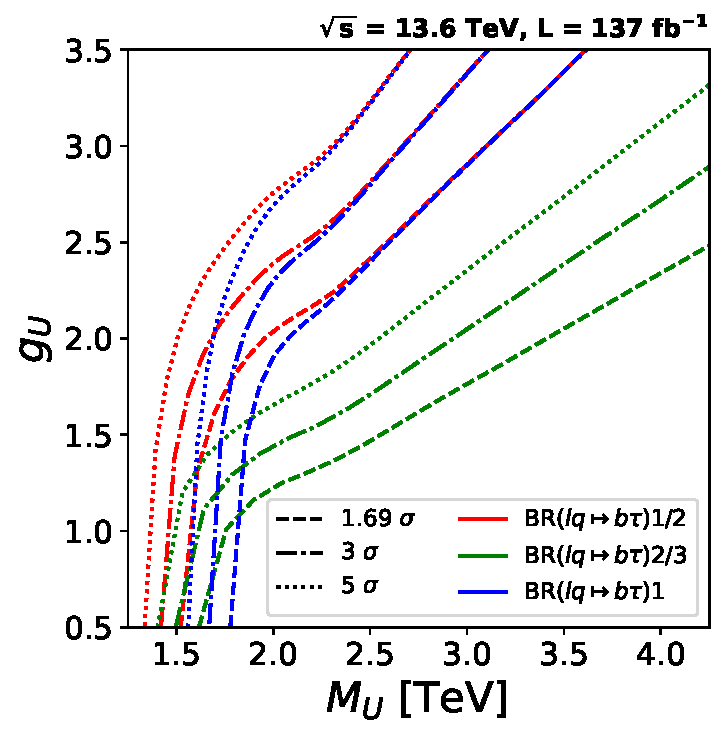
\includegraphics[height=6.5cm]{Images/Significance/Significance_Curves_Summary_by_BR.pdf}
    \caption{Signal significance for different coupling scenarios and $\lq$ masses, 
    considering the case without coupling to right-handed currents ${\rm BR}(\lq \to \bq\,\tau) = \tfrac{1}{2}$, the case maximally coupled to right- and left-handed currents ${\rm BR}(\lq\to b\,\tau) = \tfrac23$, and the case uniquely coupled to right-handed currents ${\rm BR}(\lq \to \bq\,\tau) = 1$. The estimates are performed at $\sqrt{s} = 13 \tev$ and $137 \fb^{-1}$.}
    \label{fig:combinedsigniBRs}
\end{figure}


The combined significance contours for the different ${\rm BR}$ scenarios that have been considered is presented in Fig.~\ref{fig:combinedsigniBRs}. These contours illustrate the regions of exclusion for the three cases of interest, namely exclusive left-handed currents (${\rm BR}(\lq \to \bq\,\tau) = \tfrac{1}{2}$, $\beta_R=0$), maximal left and right couplings (${\rm BR}(\lq\to b\,\tau) = \tfrac23$, $\beta_R=-1)$, and exclusive right-handed currents (${\rm BR}(\lq \to \bq\,\tau) = 1$, $g_U\to0,\,g_U\beta_R=1$). For small $g_U$, we find that the exclusive right-handed scenario is most sensitive, while the exclusive left-handed case is the worst. The reason for this is that this region is excluded principally by d$\lq$ production, such that having the largest branching ratio is crucial in order to have a large number of events. For larger couplings, both exclusive scenarios end up having similar exclusion regions, with the $\beta_R=-1$ case being significantly more sensitive. The reason in this case is that the exclusion is dominated by non-res, which has a much larger production cross-section if both currents are turned on.


\begin{figure}[]
    \centering
    \begin{subfigure}[b]{0.495\textwidth}
        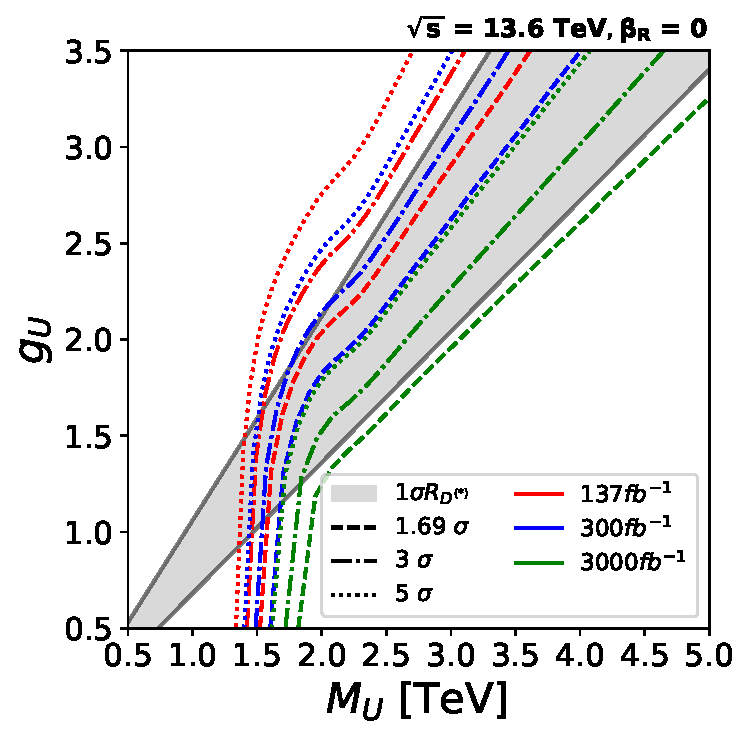
\includegraphics[height=6.5cm,]{Images/Significance/Significance_Projections_woRHC.pdf}
    \end{subfigure}
    \begin{subfigure}[b]{0.48\textwidth}
        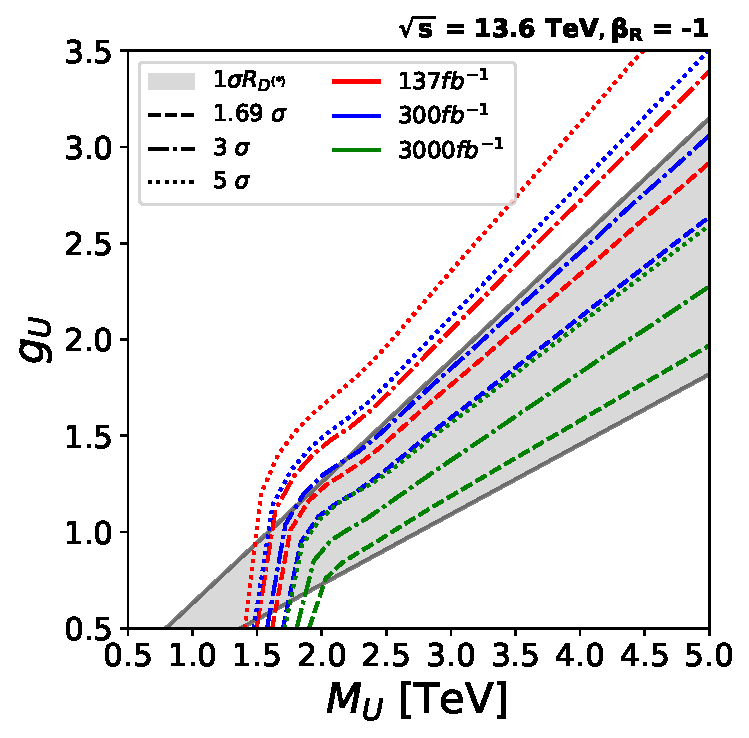
\includegraphics[height=6.5cm]{Images/Significance/Significance_Projections_wRHC.pdf}
    \end{subfigure}
    \caption{Projected signal significance for different coupling scenarios and $\lq$ masses maximally coupled to right-handed currents. The estimates are performed at $\sqrt{s} = 13.6 \tev$, $137 \fb^{-1}$, $300 \fb^{-1}$ and $3000 \fb^{-1}$.}
    \label{fig:combinedsigniLumis}
\end{figure}

In order to finalise our analysis of the LQ-only model, we show in Fig.~\ref{fig:combinedsigniLumis} the expected combined significance in the relatively near future. For this, considering $\sqrt{s} = 13.6 \tev$, we show contours for the sensitivity corresponding to integrated luminosities of $137 \fb^{-1}$,  $300 \fb^{-1}$, and $3000 \fb^{-1}$, for scenarios with only left-handed currents (top) and with maximal coupling to right-handed currents (bottom). Note that for $\beta_R = 0$ ($\beta_R = -1$), couplings $g_U$ close to 3.18 (1.85)  and $M_U = 5.0 \tev$ can be excluded with $1.69 \sigma$ significance for the high luminosity LHC era, allowing us to probe the practically the entirety of the B-meson anomaly favored region. Note that the background yields for the high luminosity LHC might be larger due to pileup effects. Nevertheless, as it was mentioned in Sec.~\ref{sec:strategyandsimulation}, we have included a conservative 10\% systematic uncertainty associated with possible fluctuations on the background estimations. Although effects from larger pileup might be significant, they can be mitigated by improvements in the algorithms for particle reconstruction and identification, and also on the data-analysis techniques.

As commented on the Introduction, non-res production can be significantly affected by the presence of a companion $\zb'$, which provides additional s-channel diagrams that add to the total cross-section and can interfere destructively with the $\lq$ t-channel process (see Figures~\ref{fig:xsinterference}
and~\ref{fig:interference}). From our previous results, we see that non-res always is of high importance in determining the exclusion region, particularly at large $M_U$ and $g_U$, meaning it is crucial to understand how this role is affected in front of a $\zb'$ with similar mass.

\begin{figure}[]
\centering
    \begin{subfigure}[b]{.48\linewidth}
    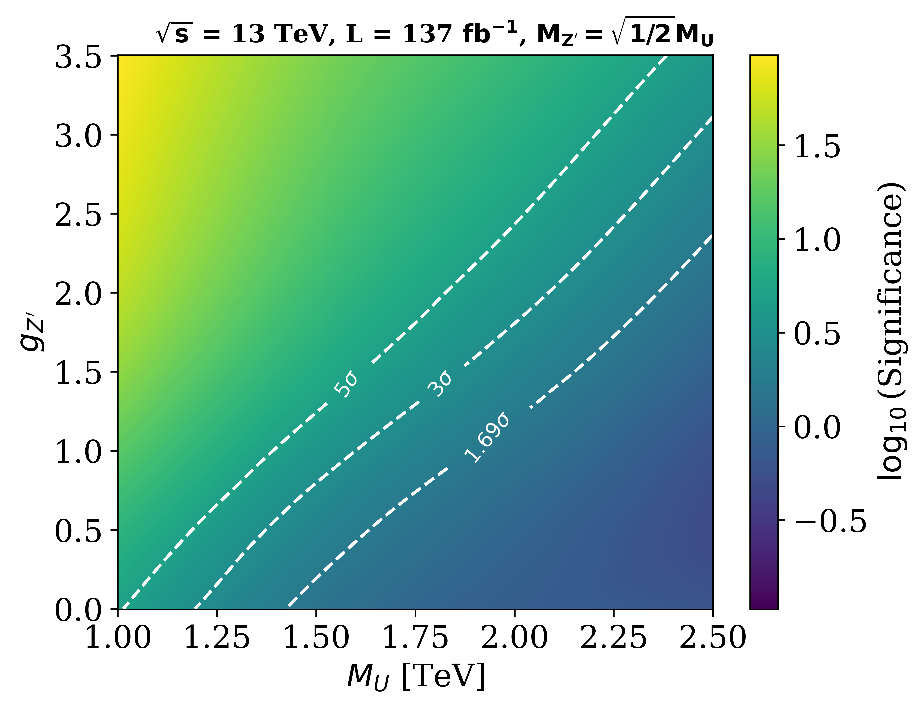
\includegraphics[height=6.1cm]{Images/Significance/zp_lower_limit_woRHC_gu1_75.pdf}
    \end{subfigure}
    \begin{subfigure}[b]{.48\linewidth}
    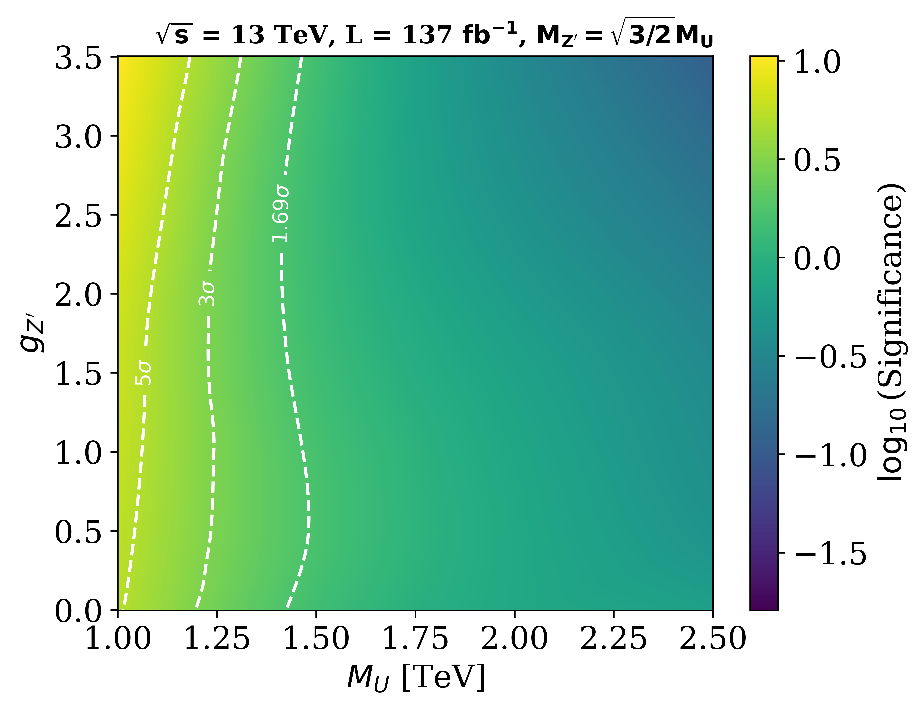
\includegraphics[height=6.1cm]{Images/Significance/zp_upper_limit_woRHC_gu1_75.pdf}
    \end{subfigure}
    \caption{Change on the non-res signal significance for different $Z^{\prime}$ coupling scenarios and $\lq$ masses. The estimates are performed at $\sqrt s=13.0 $\tev, $\beta_R=0$, $g_U = 1.8$, $M_{\zb^{\prime}} = \sqrt{1/2} M_{U}$ (top), and $M_{\zb^{\prime}} = \sqrt{3/2} M_{U}$ (bottom).}
\label{fig:sensitivity_change}
\end{figure}

The change in sensitivity on the non-res signal significance due this interference effect with the $\zb^{\prime}$ boson is shown in Fig.~\ref{fig:sensitivity_change}. We consider two opposite cases for the $\zb'$ mass: $M^2_{\zb'} = M^2_U/2$ (top) and $M^2_{\zb'} = 3\,M^2_U/2$ (bottom). Our results are shown on the $g_{\zb'}$ - $M_U$ plane, for a fixed $g_U=1.8$ and $\beta_R=0$. For the $M^2_{\zb'} = M^2_U/2$ scenario, there is an overall increase in the total cross-section, with a larger $g_{\zb'}$ implying a larger sensitivity. This means that our ability to probe smaller values of $g_U$ could be enhanced, as a given observation would be reproduced with both a specific $g_U$ and vanishing $g_{\zb'}$, or a smaller $g_U$ with large $g_{\zb'}$. Thus, for a large enough $g_{\zb'}$, it could be possible to enhance non-res to the point that the entire region favoured by $\Bm$-anomalies could be ruled out. In contrast, for $M^2_{\zb'} = 3\,M^2_U/2$ the cross-section is strongly affected by the large destructive interference, such that a larger $g_{\zb'}$ does not necessarily imply an increase in sensitivity. In fact, as can be seen in the bottom panel, for large $M_U$ the significance is reduced as $g_{\zb'}$ increases, leading to the opposite conclusion than above, namely, that a large $g_{\zb'}$ could reduce the effectiveness of non-res.

The impact of the above can be seen in Fig.~\ref{fig:sensitivity_gzp_fixed}, which shows our previous sensitivity curves on the $M_U-g_U$ plane, but this time with a $\zb'$ contribution to non-res. We use the same values of $M_{\zb'}$ as before, but fix $g_{\zb'}=3.5$. For smaller $M_{\zb'}$ (top), the non-res contribution is enhanced so much, that both s$\lq$ and d$\lq$ play no role whatsoever in determining the exclusion region. We find that, for small $g_U$, the sensitivity is dominated by $\zb'$ production such that, since $M_U$ is related to $M_{\zb'}$, $\lq$ masses up to $\sim3\tev$ are excluded. This bound is slightly relaxed for larger values of $g_U$, which is attributed to destructive interference effects due to an increased $\lq$~contribution.

\begin{figure}[]
\centering
    \begin{subfigure}[b]{.48\linewidth}
    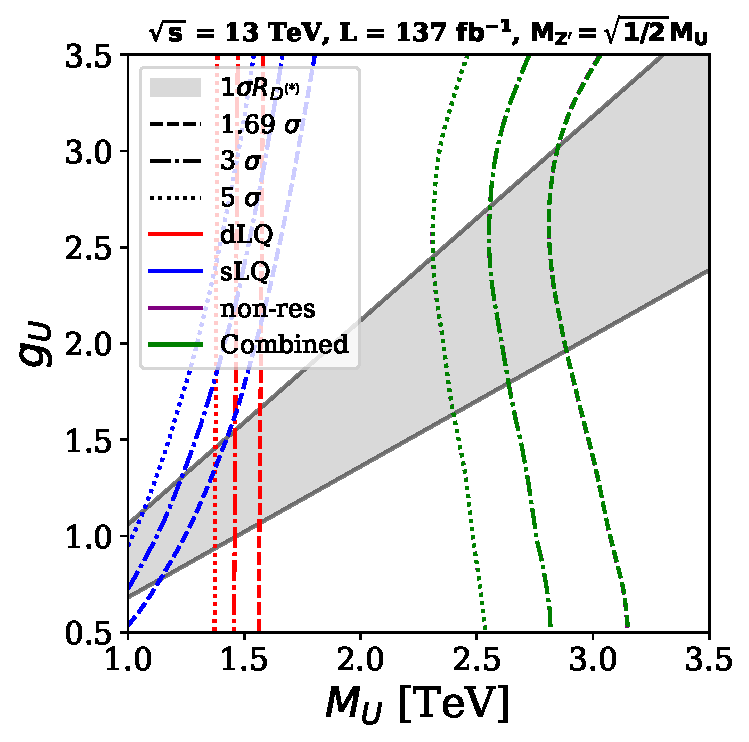
\includegraphics[height=6.1cm, width=6cm]{Images/sig_gzp_fixed/zp_lower_limit.pdf}
    \end{subfigure}
    \begin{subfigure}[b]{.48\linewidth}
    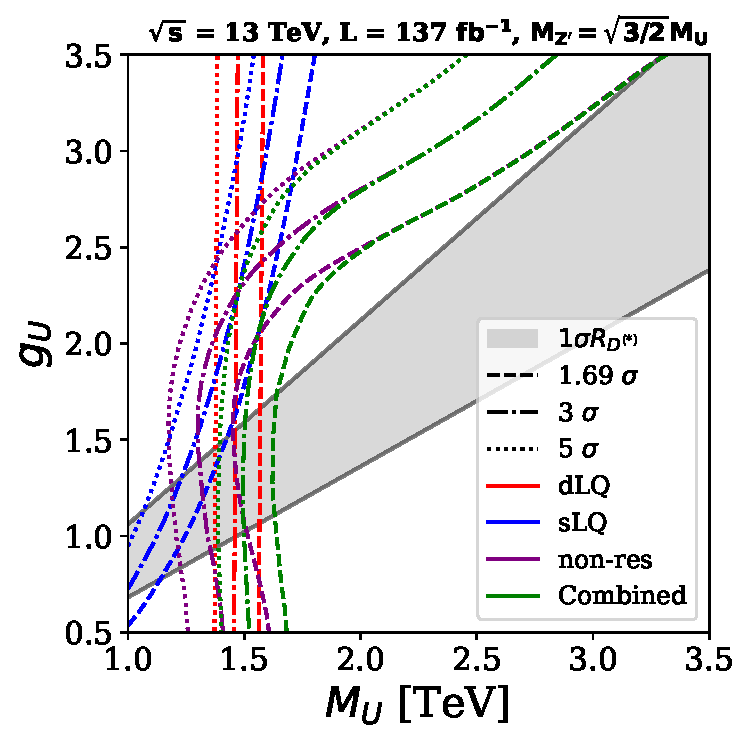
\includegraphics[height=6.1cm, width=6cm]{Images/sig_gzp_fixed/zp_upper_limit.pdf}
    \end{subfigure}
    \caption{Signal significance for different coupling scenarios and $\lq$ masses, for all channels, with an additional $\zb'$ contribution to non-res production. We set $\beta_{R} = 0$ and $g_{\zb'}=3.5$, taking $M^2_{\zb'}$ equal to $M_U^2/2$  ($3M_U^2/2$) on the top (bottom) panel.}
\label{fig:sensitivity_gzp_fixed}
\end{figure}

The bottom panel of Fig.~\ref{fig:sensitivity_gzp_fixed} shows that case where $M_{\zb'}$ is larger than $M_U$. As expected from our previous discussion, the behaviour and impact of non-res is modified. For small $g_U$, we again have the pure $\zb'$ production dominating the non-res cross-section, leading to a null sensitivity on $g_U$, similar to what happens in dLQ. In contrast, for very large $g_U$, we find that the pure $\lq$ non-res production is the one that dominates, and we recover sensitivity regions with a slope similar to those shown in Figures~\ref{fig:heatmapssignificance}-\ref{fig:combinedsigniLumis}, shifted towards larger values of $g_U$. For intermediate values of this coupling, the destructive interference have an important effect again, twisting the exclusion region slightly towards the left. Still, even in this case, we find that s$\lq$ plays a marginal role in defining the combined exclusion region, and that the final result again depends primarily on d$\lq$ and non-res production.